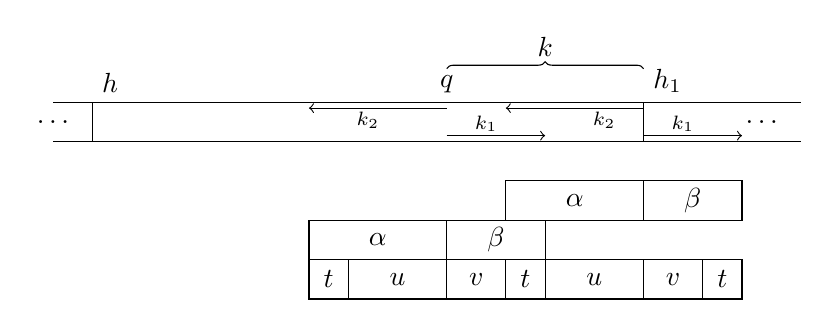
\begin{tikzpicture}[scale=0.5]
    %Boite supérieur et indice
    \draw (-2,0)--(17,0);
    \draw (-2,1)--(17,1);
    \draw (-1,1)--(-1,0);
    \draw (13,1)--(13,0);
    \node at (-2,0.5) {$\dots$};
    \node at (16,0.5) {$\dots$};
    \node[above right] at (-1,1) {$h$};
    \node[above right] at (13,1) {$h_1$};
    \node[above] at (8,1) {$q$};
    \draw[decoration={brace,raise=5pt},decorate]
    (8,1.5) -- node[above=6pt] {$k$} (13,1.5);
    %Flèche pour $k_i$
    \draw[->] (13,0.85)--(9.5,0.85);
    \node[below] at (12,1) {\scriptsize $k_2$};
    \draw[->] (8,0.85)--(4.5,0.85);
    \node[below] at (6,1) {\scriptsize $k_2$};
    \draw[->] (13,0.15)--(15.5,0.15);
    \node[above] at (9,0) {\scriptsize $k_1$};
    \draw[->] (8,0.15)--(10.5,0.15);
    \node[above] at (14,0) {\scriptsize $k_1$};
    %Facteur alpha beta
    \draw (13,-1) rectangle (9.5,-2) node[pos=.5] {$\alpha$};
    \draw (8,-2) rectangle (4.5,-3) node[pos=.5] {$\alpha$};
    \draw (13,-1) rectangle (15.5,-2) node[pos=.5] {$\beta$};
    \draw (8,-2) rectangle (10.5,-3) node[pos=.5] {$\beta$};
    %Facteur w,u,t
    \draw (10.5,-3) rectangle (9.5,-4) node[pos=.5] {$t$};
    \draw (10.5,-3) rectangle (13,-4) node[pos=.5] {$u$};
    \draw (8,-3) rectangle (9.5,-4) node[pos=.5] {$v$};
    \draw (4.5,-3) rectangle (5.5,-4) node[pos=.5] {$t$};
    \draw (8,-3) rectangle (5.5,-4) node[pos=.5] {$u$};
    \draw (13,-3) rectangle (14.5,-4) node[pos=.5] {$v$};
    \draw (14.5,-3) rectangle (15.5,-4) node[pos=.5] {$t$};
\end{tikzpicture}